\begin{minipage}{0.45\textwidth}
\centering
\begin{tikzpicture}[font=\small,declare function={fx(\r,\t)=\r*cos(\t);fy(\r,\t)=\r*sin(\t);fz(\r,\t)=9-(\r)^2;g(\x,\y)=14-2*\x-4*\y;}]
\pgfmathsetmacro{\ra}{1}
\pgfmathsetmacro{\ang}{300}
\begin{axis}[view/h=115,clip=false,axis lines=center,small,colormap={}{gray(0cm)=(0.6);gray(1cm)=(0.9);},enlargelimits=true,xlabel={$x$},ylabel={$y$},zlabel={$z$},xlabel style={anchor=north},ylabel style={anchor=west},zlabel style={anchor=south},xtick={\empty},ytick={\empty},ztick={\empty}]
%\addplot3[surf,z buffer=sort,domain=-1:1,domain y=-1:1]{f(x,y)};
\addplot3[surf,z buffer=sort,domain=0:3,domain y=0:360]({fx(x,y)},{fy(x,y)},{fz(x,y)});
\addplot3[surf,domain=-0.75:2.25,domain y=1:3]{g(x,y)};
\addplot3[]coordinates{(-0.75,1,{g(-0.75,1)})}node[right]{\RL{مماسی مستوی}};
\addplot3[]coordinates{({fx(\ra,\ang)},{fy(\ra,\ang)},{fz(\ra,\ang)})}node[above left]{\RL{دائری قطع مکافی}};
\addplot3[]coordinates {(1,2,4)(1+2,2+4,4+1)}node[pos=0,circ]{}node[pos=0,above,font=\scriptsize]{$N_0(1,2,4)$}node[right,yshift=1ex]{\RL{عمودی خط}};
\end{axis}
\end{tikzpicture}
\caption{نقطہ \عددی{N_0} پر دائری قطع مکافی سطح   کا مماسی مستوی اور عمودی خط (مثال \حوالہ{مثال_کثیرالمتغیر_عمودی_خط_مماسی_مستوی_دائری_قطع_مکافی})۔}
\label{شکل_مثال_کثیرالمتغیر_عمودی_خط_مماسی_مستوی_دائری_قطع_مکافی}
\end{minipage}
+++++++++++++++++++++++++++++++++++++++++++++++++++++++++++++++++
=======================================================================
\begin{minipage}{0.45\textwidth}
\centering
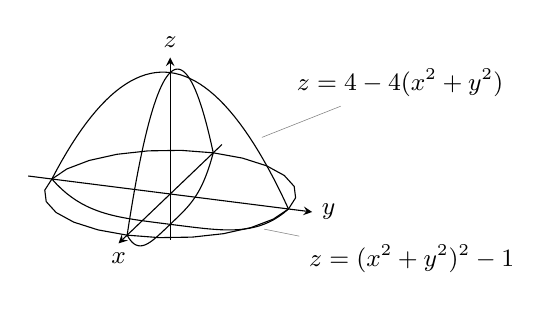
\begin{tikzpicture}[font=\small,declare function={fx(\r,\p)=\r*cos(\p);fy(\r,\p)=\r*sin(\p);fz(\r,\p)=4-4*\r^2;fzz(\r,\p)=\r^4-1;}]
\pgfmathsetmacro{\pa}{0}
\pgfmathsetmacro{\pb}{90}
\pgfmathsetmacro{\pc}{180}
\pgfmathsetmacro{\pd}{270}
\pgfmathsetmacro{\tp}{110}
\pgfmathsetmacro{\tpa}{180+\tp}
\begin{axis}[clip=false,view/h=110,small,axis lines=middle,xtick={\empty},ytick={\empty},ztick={\empty},enlargelimits=true, xlabel={$x$}, ylabel={$y$},zlabel={$z$}, xlabel style={anchor=north},ylabel style={anchor=west},zlabel style={anchor=south},colormap={}{gray(0cm)=(0.6);gray(1cm)=(0.9);}]
\addplot3[black,domain=0:1,variable=\r, variable y=\p,samples y=0]({fx(r,\pa)},{fy(r,\pa)},{fz(r,\pa)});
\addplot3[black,domain=0:1,variable=\r, variable y=\p,samples y=0]({fx(r,\pb)},{fy(r,\pb)},{fz(r,\pb)})node[pos=0.5,pin=45:{$z=4-4(x^2+y^2)$}]{};
\addplot3[black,domain=0:1,variable=\r, variable y=\p,samples y=0]({fx(r,\pc)},{fy(r,\pc)},{fz(r,\pc)});
\addplot3[black,domain=0:1,variable=\r, variable y=\p,samples y=0]({fx(r,\pd)},{fy(r,\pd)},{fz(r,\pd)});
\addplot3[black,domain=0:1,domain y=0:360,variable=\r, variable y=\p]({fx(1,p)},{fy(1,p)},{fz(1,p)});
\addplot3[black,domain=0:1,variable=\r, variable y=\p,samples y=0]({fx(r,\pa)},{fy(r,\pa)},{fzz(r,\pa)});
\addplot3[black,domain=0:1,variable=\r, variable y=\p,samples y=0]({fx(r,\pb)},{fy(r,\pb)},{fzz(r,\pb)})node[pos=0.5,pin=-10:{$z=(x^2+y^2)^2-1$}]{};
\addplot3[black,domain=0:1,variable=\r, variable y=\p,samples y=0]({fx(r,\pc)},{fy(r,\pc)},{fzz(r,\pc)});
\addplot3[black,domain=0:1,variable=\r, variable y=\p,samples y=0]({fx(r,\pd)},{fy(r,\pd)},{fzz(r,\pd)});
\end{axis}
\end{tikzpicture}
\caption{جسم برائے شکل \حوالہ{سوال_بالکثرت_ٹھوس_جسم_حجم_الف}}
\label{شکل_سوال_بالکثرت_ٹھوس_جسم_حجم_الف}
\end{minipage}\hfill
======================================================

\begin{minipage}{0.3\textwidth}
\centering
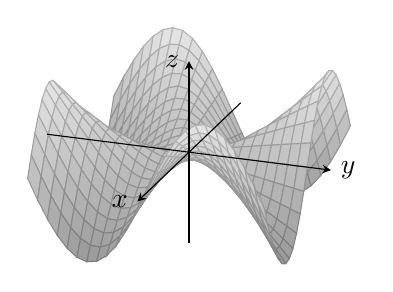
\begin{tikzpicture}[declare function={f(\x,\y)=\x*\y*((\x)^2-(\y)^2)/((\x)^2+(\y)^2);}]
  \begin{axis}[axis on top,view/h=110,small,axis lines=center,colormap={kgray}{gray(0.2cm)=(0.6);gray(1cm)=(0.9);},xtick={\empty},ytick={\empty},ztick={\empty},enlargelimits=true,xlabel={$x$},ylabel={$y$},zlabel={$z$},xlabel style={anchor=east},ylabel style={anchor=west},zlabel style={anchor=east}]
\addplot3[surf]{f(x,y)};
\end{axis}
\end{tikzpicture}
\caption{$z=\tfrac{xy(x^2-y^2)}{x^2+y^2}$}
\end{minipage}\hfill
\begin{minipage}{0.3\textwidth}
\centering
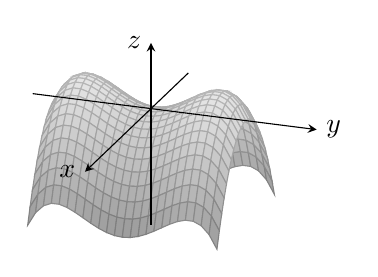
\begin{tikzpicture}[declare function={f(\x,\y)=(\y)^2-(\y)^4-(\x)^2;}]
  \begin{axis}[axis on top,view/h=110,small,axis lines=center,colormap={kgray}{gray(0.2cm)=(0.6);gray(1cm)=(0.9);},xtick={\empty},ytick={\empty},ztick={\empty},enlargelimits=true,xmax=2,ymax=1.5,zmax=0.5,xlabel={$x$},ylabel={$y$},zlabel={$z$},xlabel style={anchor=east},ylabel style={anchor=west},zlabel style={anchor=east}]
\addplot3[surf,domain=-1:1,domain y=-1:1]{f(x,y)};
\end{axis}
\end{tikzpicture}
\caption{$z=y^2-y^4-x^2$}
\end{minipage}

======================================

\begin{minipage}{0.30\textwidth}
\centering
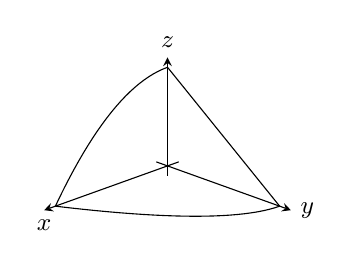
\begin{tikzpicture}[font=\small,declare function={fx(\x,\y)=\x;fy(\x,\y)=\y;fz(\x,\y)=4-\x^2-\y;}]
\begin{axis}[clip=false,view/h=135,width=5cm,axis lines=middle,xtick={\empty},ytick={\empty},ztick={\empty},enlargelimits=true, xlabel={$x$}, ylabel={$y$},zlabel={$z$}, xlabel style={anchor=north},ylabel style={anchor=west},zlabel style={anchor=south},colormap={}{gray(0cm)=(0.6);gray(1cm)=(0.9);}]
\addplot3[domain=0:2,samples y=0]({fx(x,0)},{fy(x,0)},{fz(x,0)});
\addplot3[domain=0:2,samples y=0]({x},{4-x^2},{0});
\addplot3[]coordinates{(0,4,0)(0,0,4)};
\end{axis}
\end{tikzpicture}
\caption{خاکہ برائے سوال \حوالہ{سوال_بالکثرت_خطہ_کا_حجم_درکار_ح}}
\label{شکل_سوال_بالکثرت_خطہ_کا_حجم_درکار_ح}
\end{minipage}\hfill

